% v2-acmsmall-sample.tex, dated March 6 2012
% This is a sample file for ACM small trim journals
%
% Compilation using 'acmsmall.cls' - version 1.3 (March 2012), Aptara Inc.
% (c) 2010 Association for Computing Machinery (ACM)
%
% Questions/Suggestions/Feedback should be addressed to => "acmtexsupport@aptaracorp.com".
% Users can also go through the FAQs available on the journal's submission webpage.
%
% Steps to compile: latex, bibtex, latex latex
%
% For tracking purposes => this is v1.3 - March 2012

\documentclass[prodmode,acmtecs]{acmsmall} % Aptara syntax

% Package to generate and customize Algorithm as per ACM style
\usepackage[ruled]{algorithm2e}
\usepackage{cite}
\usepackage{amssymb}
\usepackage{multirow}
\usepackage{tikz}
\usetikzlibrary{mindmap,trees}
\renewcommand{\algorithmcfname}{ALGORITHM}
\SetAlFnt{\small}
\SetAlCapFnt{\small}
\SetAlCapNameFnt{\small}
\SetAlCapHSkip{0pt}
\IncMargin{-\parindent}
\setlength\parindent{0pt}
\usepackage{setspace}
%\doublespacing
\linespread{2}

% Metadata Information
\acmVolume{9}
\acmNumber{4}
\acmArticle{39}
\acmYear{2010}
\acmMonth{3}

\newcommand{\jm}[1]{
    \noindent{\textcolor{red}{\bf\em #1 -- Johan}}
}
\newcommand{\km}[1]{
    \noindent{\textcolor{blue}{\bf\em #1 -- Ketan}}
}

% Document starts
\begin{document}

% Page heads
\markboth{K. Maheshwari et al.}{A Survey of Scientific Workflow Management Systems}

% Title portion
\title{State of the Art in Scientific Workflow Systems}
\author{KETAN MAHESHWARI
\affil{University of Nice, Sophia Antipolis}
JOHAN MONTAGNAT
\affil{CNRS}
}
% NOTE! Affiliations placed here should be for the institution where the
%       BULK of the research was done. If the author has gone to a new
%       institution, before publication, the (above) affiliation should NOT be changed.
%       The authors 'current' address may be given in the "Author's addresses:" block (below).
%       So for example, Mr. Abdelzaher, the bulk of the research was done at UIUC, and he is
%       currently affiliated with NASA.

\begin{abstract}

\km{TODO: Expand in the end}

In this work we conduct a literature survey of the key features of the
contemporary scientific workflow environments. We define the criteria for the
survey based chiefly on user needs arising from diverse applications and
infrastructure. An overview of studied scientific workflow environments is
presented followed by the identification and description of the features offered by
each of the environment. A tabulated summary for each feature class gives a
high-level view of the offered features. Finally, a taxonomy is proposed
placing these features into respective places in a hierarchy. 

\jm{Test comment}

\end{abstract}
%\category{C.2.2}{Computer-Communication Networks}{Network Protocols}
%\terms{Design, Algorithms, Performance}
%\keywords{Wireless sensor networks, media access control, multi-channel, radio interference, time synchronization}

\acmformat{Ketan Maheshwari, Johan Montagnat
, 2014. A survey of scientific workflow management systems.}
% At a minimum you need to supply the author names, year and a title.
% IMPORTANT:
% Full first names whenever they are known, surname last, followed by a period.
% In the case of two authors, 'and' is placed between them.
% In the case of three or more authors, the serial comma is used, that is, all author names
% except the last one but including the penultimate author's name are followed by a comma,
% and then 'and' is placed before the final author's name.
% If only first and middle initials are known, then each initial
% is followed by a period and they are separated by a space.
% The remaining information (journal title, volume, article number, date, etc.) is 'auto-generated'.

\begin{bottomstuff}
This work is supported by the ANR-CNRS, under
grant contract CNRS-0435060.

Author's addresses: Ketan Maheshwari, Argonne National Laboratory; Johan Montagnat, I3S, Sophia Antipolis.
\end{bottomstuff}

\maketitle

%Workflows considered:
% MOTEUR2
% Taverna
% Swift
% Pegasus
% Triana % not sure
% Galaxy
% Makeflow
% Kepler/Ptolemy
% Vistrails
% Linda
% DaGue
% Wings
% PGRADE Portal

\input{text/intro}
\section{Conceptual Overview}
In this section we present a conceptual overview of the subjects of this
study--Workflows and Scientific Workflow Environments.

\subsection{Workflow}
Figure~\ref{fig:wf} shows a typical workflow in the form of a Directed Acyclic
Graph (DAG). Execution typically begins with the input data being provided to
the first task and ends at the results being delivered at the end of the last
task. Tasks are represented by boxes and data/control flow between the task is
represented as arrows. Note that in cases where tasks are connected with pure
control flow, it can be simulated by passing token data between tasks.

For the purpose of this text, we define a workflow as a specification of
computation with at least two discrete tasks either forming distinct
computational stages or running for two or more distinct datasets as
parameters. Consequently, a one-off task or running a task for a single copy of
data is \emph{not} a workflow.

For the rest of this paper, we will use the above definition of a workflow.
%

\begin{figure}[htb]
\begin{center}
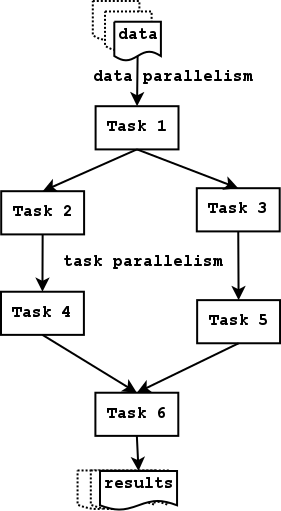
\includegraphics[width=4cm]{figures/workflow}
\caption{A typical workflow depicted as a Directed Acyclic Graph (DAG) of tasks coordinated by data or control flow and illustrating data and task parallelism}
\label{fig:wf}
\end{center}
\end{figure}
%

\subsection{Architecture}
Figure~\ref{fig:wfms} shows a high-level architecture of a generic SWE. It shows key
components and their interaction in an SWE. These components are the focus of
interest for the present work. A \textit{user interface} interacts with the
\textit{workflow engine} using commands and messages on the inside while with
user on the outside. The \textit{workflow language} becomes an intermediate
representation for communication between user interface and the
\textit{workflow engine}. The workflow engine acts as a compiler/interpreter
and a high-level scheduler for the processors and interfaces with the
underlying \textit{distributed resources}. It resolves data dependencies and
optimizes the flow at runtime and monitors the workflow progress and collects
the intermediate and final results.

%
\begin{figure}[htb]
\begin{center}
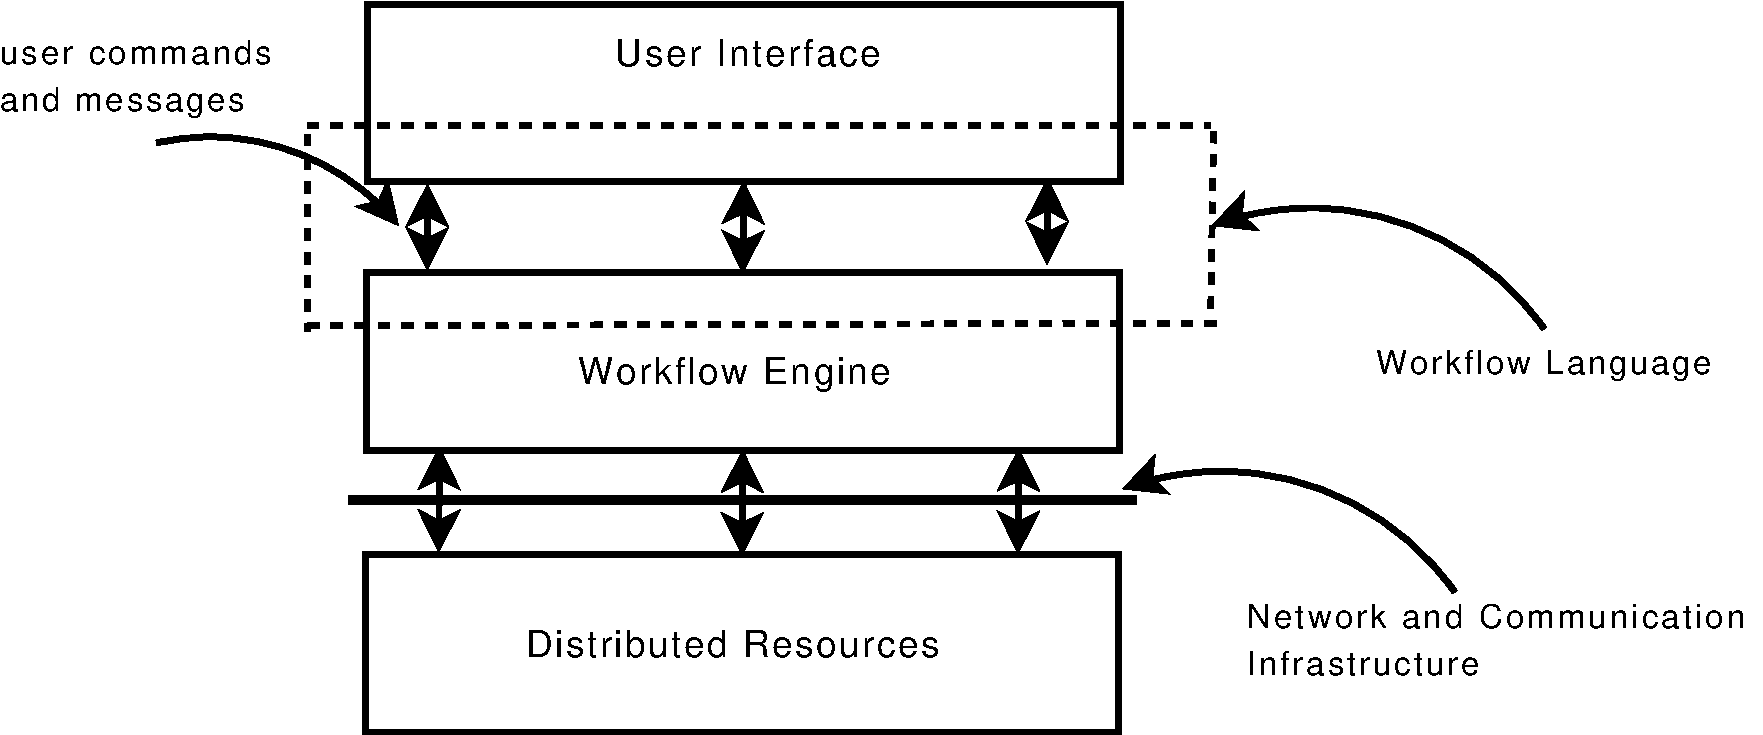
\includegraphics[width=\linewidth]{figures/workflow_interfaces_and_language}
\caption{A generic SWE scheme showing the relationship and interaction among important components}
\label{fig:wfms}
\end{center}
\end{figure}
%
SWEs are used as tools to benefit from the underlying large-scale computing
infrastructure such as clusters, supercomputers, clouds, and grids. Such
environments are in use today for production level work in different scientific
domains worldwide. They do the basic task of linking inter-related processors
of a multi-staged scientific computation. However, they differ in the features
they provide based upon the scientific domain or user community they offer
service for, and the computational model they follow. Often, one of the main
reasons for such difference is the specialized components and requirements for
a particular domain. Owing to this fact, a given workflow system dominates a
particular area of science (eg. astronomy, biology, etc.). Nonetheless, there
exist a plethora of SWEs suitable for general purpose workflow style
computations.

DAGs are by far, the most popular abstraction of the way workflows are
perceived and visualized. The MA DAG~\cite{caron-desprez:2005}, engine is one
example of a DAG generator engine. MA DAG has evolved from a regular DAG
generator to a more abstract DAG generator laced with control structures. MA
DAG benefits from the workflow scheduling mechanisms included in the
middleware. Due to the impossibility to produce complete DAGs owing to the
presence of control structures such as conditionals and loops, MA DAG generate
partial DAGs greedily: a sub-DAG, as complete as possible, is produced as soon
as possible. Despite the presence of many different approaches to workflow
systems, new requirements continue to pose workflow challenges. Some of the
current challenges facing SWEs are:

\begin{enumerate}
\item \textbf{Multisite execution.} Interfacing to existing computation and
storate infrastructure is not trivial, not to mention the new and
unforeseen access and compute modes. SWEs are yet to formulate a
generalized interface towards the major platforms such that they will
run on them out of the box.

\item \textbf{Manysite execution.} Even if a SWE has interfaces built for
more than one infrastructure, it is hard to optimally schedule large
workflows to many remote sites simultaneously. The problem of limited
control over remote sites and distributing interdependent data and
tasks makes it non-trivial to efficiently load-balance work among them.

\item \textbf{Expressivity.} Workflow languages have evolved over the years
with reasonable expressivity being supported. However, they are often
compared with those of the traditional programming languages. As of
current state of the art, the workflow languages expressivity still
have to catch up to the richness of programming languages across
different generations such as C and python.  The community is yet to
realize a truly generic workflow language that can express a wide
variety of flow patterns encountered in scientific domains.

\item \textbf{Interoperability.} Interoperable workflows will benefit to a
broad audience of users. Many efforts at this are made in the recent
past, such as by the consurtium projects and by individual players.
However, a truly interoperable set of standards for workflows are yet
to emerge.
\end{enumerate}

\section{Related Work}
Surveys and studies on workflows similar to the present one have been done in
the past. Yu and Buyya \cite{yu-buyya:2005} proposed a detailed taxonomy of
SWEs in the previous decade, studying many existing systems for distributed
computing. This taxonomy presented is based, to a large extent on the
capabilities of the workflow engines. It does provide insights to many of the
SWE aspects considered in the present paper, especially the workflow languages
expressiveness and SWEs interactions with the distributed computing
infrastructures in the early days of the compute Grids. A more recent work by
Goderis \cite{goderis-brooks-etal:2009} studies a topic more closely related to
the workflow language expressiveness: it compares the models of computations of
various workflow directors implemented in Kepler
\cite{ludascher-altintas-etal:2005a} with the perspective of enabling
composition of different models in sub-workflows of a global orchestration.
This work illustrates how different enactors designed for different application
needs have different expressiveness power. Deelman et. al.
\cite{deelman-overview} present a high-level overview of the scientific
workflow features and capabilities including SWE composition, representation
and resource mapping capabilities. A recent survey from
Stratan~\cite{stratan-iosup-etal:2008} about the workflow engine performance
takes into account the latencies involved during the enactment mechanisms. A
small survey and analysis of file-access characteristics for data-intensive
workflows has been done by Shibata~\cite{Shibata}. Early surveys on workflow
languages and suitability of general purpose languages to workflows is
conducted in~\cite{generalpurpose}. These surveys were conducted before a few
years and in the meantime SWEs have come a long way in terms of capabilities
and enactment approaches. New techniques such as the map/reduce framework
\cite{mapreduce} have been introduced as a promising new approach to workflow
enactment over distributed infrastructures. Several issues put forth by such
surveys such as customized service wrapping and enactment have been adequately
addressed over the
years~\cite{glatard-montagnat-etal:2008a,rojasbalderrama-montagnat-etal:2010}.

Another well-studied feature is the workflow languages. Many different
languages have been considered within the SWE community, from raw Directed
Acyclic Graphs (DAGs) of computational processes such as CONDOR
DAGMan~\cite{dagman} to abstractions for parallel computations such as Petri
nets~\cite{alt-hoheisel:2005}, data-driven languages such as
Scufl~\cite{turi-missier-etal:2007} and scripting languages such as Swift
script~ \cite{swift}. Glatard's PhD thesis~\cite{glatard:2007} presents a
taxonomy of SWE languages classifying them into functional, graph,
service-oriented and executable representations. A detailed classification and
taxonomy of parallelism patterns in Grid Workflows has been presented by
Pautasso and Alonso in~\cite{pautasso1}. This classification is more generic
while the one presented in Glatard's thesis has emphasis on service based
workflows.  Each of these approaches can be defended through some aspects well
covered in their design: DAGs are convenient for scheduling
\cite{Malewicz:2007,hall-rosenberg-etal:2007}, Petri nets can be used to detect
properties such as potential deadlocks, data-driven languages ease the
description of application logic for non-expert users and scripting is
extensively used by programmers for prototyping, etc.

\section{Objectives and Organization}
% What are the goals of this work?
% How is this paper supposed to help:
% -- Existing scientific users who have not adopted workflows
% -- Existing users who have adopted workflows
% -- New users
% -- Experts in the field

% Say that different workflow systems have different design goals. It is hard
% to chose one from the existing or build your own. It is almost equally
% complex to build own just as it is complex to create own programming
% platform. We hope to provide by the way of this paper a guide for new adopters on how to chose a workflow language appropriate for their needs. We ask and answer the following questions of the workflow systems that we study in this paper:
%-- What were the original design goals?
%-- What are the main application areas that the system is currently being used?
%-- What are the characteristics and capabilities of the language? expressivity features?
%-- What are the characteristics and capabilities of the run-time? parallelism? concurrency? task and data grouping?
%-- What kinds of computing and computational infrastructure does the workflow system cater to? Grids, Clouds, Clusters, Supercomputers, fast IB networks? Accelerators?
%-- How have they evolved? What are the possible future directions?

In the present work we survey and study the various contemporary SWEs in order
to find the capabilities and key features in terms of the characteristics
described in section~\ref{sec:intro}. We believe this study will serve to
address the following objectives:

\begin{enumerate}
\item \textbf{Educate.} With more science being done with the help of
computational methods, SWEs can add significant value to the process.  They can
accelerate the process, enable community driven science, drive the development
at a manageable level of abstraction for users.  However, scientific users are
often not experienced programmers or computation savvy. This work will serve as
a useful starting guide to educate science users and students of the available
tools and techniques with features suitable for their methods.

\item \textbf{Catalog.} We study a number of important features as offered by
the contemporary SWEs. This will help catalog and collect the SWEs by their
offerings and identify mechanisms and needs for new and existing features
in one place. This will also help identify current trends and approaches
to computation in scientific communities.

\item \textbf{Application.} We identify the applications and application
classes well adapted to the workflow systems and are benefitting by them.
This will help readers relate to the application they are associated to.
We hope that readers can make a choice of which SWE to use if there is an
adaptation similar in scope to the ones describe in this paper.

\item \textbf{Evolution.} We comment on the evolution of the existing workflow
systems and the possible current and future development directions which
will help readers be aware of the general development direction of the
SWEs.
\end{enumerate}

The rest of this paper is organized as follows: Section
\ref{sec:overview} presents an overview of the key SWEs studied in this work.
Section \ref{sec:scal} discusses the optimization features and resulting
scalable performance as observed in the SWEs studied. Section \ref{sec:data}
studies the data management and description aspects of the SWEs. Section
\ref{sec:inter} presents a study of SWEs approaches to interface the
large-scale computing infrastructures. Section \ref{sec:lang} details the
language features and expressiveness of the SWEs studied. Section
\ref{sec:usable} discusses the usability aspects of the SWEs.  Section
\ref{sec:sum} presents a summary and a classification of all the aspects of
SWEs studied in this work. 

Throughout the paper, we also present tables
summarizing the aspects of SWEs considered in respective sections. It was not
possible to obtain an exhaustive information about all the SWEs considered in
this work. We rely on the following sources for our information: 
\begin{enumerate}
    \item \textbf{Publications.} Peer reviewed publications in journals, conferences and workshops.
    \item \textbf{Technical Reports.} Technical reports and theses.
    \item \textbf{Web Presence.} Documentation and other information from the web pages hosting the SWE.
    \item \textbf{Experience.} Where possible, we tried features of the SWEs by installing them on the available systems. 
\end{enumerate}

Some features, such as extendability of an SWE strongly depend on the extension
points designed in the code; consequently, we consider it present in only those
SWEs that have an explicit documented description or demonstration of the given
feature. 


%Confusion over the use of Workflows in HPC community and supercomputing centers.

\section{Overview of the Workflow Environments} \label{sec:overview}
In this section we present an overview of the SWEs studied. The paragraph
headers are organized by the name of the SWE followed by the name of internal
representation language use and support separated by a forward slash (/).  The
cases where an intermediate language is not specifically defined or conversely
where there are multiple systems supporting a generic representation are
denoted by an asterisk (*) or a hyphen (-) at the respective places.

\paragraph{Taverna/scufl} The Taverna Workflow Management System
\cite{taverna2013} is an open source scientific dataflow manager
developed by the mygrid~consortium in the UK.
%
Taverna includes a GUI-based rich-client workbench for workflow design and a
workflow enactment runtime. Taverna can enact workflows expressed in the scufl
language. Scufl is a near Turing complete dataflow language with well-defined
semantics \cite{turi-missier-etal:2007,glatard-montagnat:2008}. 

A Taverna workflow consists of a collection of processors connected by data and
coordination links, which establish a dependency between the output(s) of a
processor and the input(s) of another. The processors are of different kinds
depending on the application code to be invoked: typically being services, with
input and output \textit{ports} that correspond to the operation's invocations
and response sequences defined in the service`s interface expressed as REST or WSDL.
Java classes and local scripts can be used as workflow processors, as long as
they expose their signature as input and output ports as required by the model.
The engine orchestrates the execution of the processors in a way that is
consistent with the dependencies, and manages the flow of data through the
processors' ports. The overall workflow execution is data-driven, with a
\emph{push} model: a processor's execution is started as soon as all of its
inputs are available. Taverna is a flexible and extendible workflow environment
\cite{missier-soiland-reyes-etal:2010,sroka2009a} in that extending the
engine's functionality is facilitated through a Service Provider Interface
(SPI). The Taverna engine implements a sophisticated mechanism for enactment of
parallel workflows. These mechanisms manifest in the form of complex pipelines
and an advanced superpipelined enactment of workflows. Such a mechanism induces
multiple downstream workflow processors running in parallel for a dataset. In
the case of superpipelines, multiple pipeline instances run for multi-datasets
providing a high degree of parallelism limited only by the availability of
underlying resources. Taverna is not natively interfaced with external
computational infrastructure but the same can be achieved with the help of
extending the engine through one of its
SPIs~\cite{maheshwari-missier-etal:2009}. In a crucial development, recent
implementations of Taverna offers a client-server based environment in which a
Taverna \emph{server} can remotely serve the workflow composition and execution
services. This mode is useful in the cloud computing environments where the
server decides where to run the Taverna services in the cloud.

\paragraph{MOTEUR/scufl, GWENDIA} MOTEUR \cite{glatard-montagnat-etal:2008} is a SWE
developed at the I3S laboratory, University of Nice at Sophia Antipolis (UNS).
MOTEUR facilitates executing workflows consisting of remote services. It
exploits service parallelism at workflow level and data parallelism for
multiple datasets. 

MOTEUR has sophisticated language-level expressions for data management
mechanisms within a workflow definition. It provides a diverse set of
parallel iterators that are well adapted for different combinations of input datasets
at the processor. An iteration strategy allows different combinations of the
data arriving at a processor along its multiple inputs. Running legacy
application code on distributed systems has been eased by MOTEUR by providing a
generic grid-service wrapper for these applications
\cite{glatard-montagnat-etal:2008a}. Services thus created can be readily
deployed by the MOTEUR runtime. MOTEUR workflows are written in the scufl
language and are compatible with those written for the Taverna SWE. It also
supports an extension of scufl language called the Gwendia~\cite{gwendia}
language, developed at the same laboratory. 
%

\paragraph{Makeflow/make-like spec} Makeflow~\cite{makeflow} is a make-like workflow platform.
Makeflow addresses the often-encountered problem of software and library
dependencies on workflow tasks execution for heterogeneous environments.
Makeflow offers techniques to ``link" and package the application execution
elements such as executables, libraries and configuration parameters. This
improves the durability of a workflow and decreases the efforts required to
maintain a working version of an application encoded as a workflow.

%Internal representation of a Makeflow workflow is in...
%Its expressivity features include...
%Makeflow's runtime features include...
%

%\paragraph{Triana/XML} Triana \cite{taylor-shields-etal:2003} is a java-based
SWE developed at the Cardiff University. It consists of a workflow composition
GUI, a framework to integrate workflow with the different execution
environments and middlewares and a set of predefined services written as java
components. A Triana workflow is expressed as an XML grammar similar to a WSDL
description for webservices \cite{taylor-wand-etal:2005}. A highlight of
Triana is that it provides ready-to-use interface for a wide variety of
middleware and distributed infrastructures including P2P, grids and
web-services frameworks. A Triana workflow provides dataflow as well as control
flow support. Triana allows conditional branching and looping in its workflows.

\input{text/vistrails}
\paragraph{Kepler/MoML} Kepler~\cite{kepler2013} is a SWE
based upon the Ptollemy II framework~\cite{eker-janneck-etal:2003} developed at
the University of California. Kepler workflows follow an actor-director
metaphor where an actor represents a processor and the director
represents the paradigm for executing the workflows consisting of the actors.
Depending upon the types of directors, a Kepler workflow may exhibit a
different type of execution behavior. A workflow designer can chose from among
directors based upon the purpose of a workflow. Few of these include Process
Network (PN) for a parallel execution at the workflow level, Synchronous Data
Flow (SDF) for simple sequential data flow and Collection Oriented Modeling and
Design (COMAD) \cite{keplercomad} for a collection oriented workflow. Kepler
uses the Modeling Markup Language (MoML) for its workflow representation. MoML
is an extended XML syntax providing a rich vocabulary to compose Kepler
workflows. A workflow processor is called an `actor' in Kepler. Recent advances
in Kepler include MapReduce style computation, bioinformatics computation,
cloud computing~\cite{kepler2013}.

%
\paragraph{Pegasus/DAX} Pegasus \cite{deelman-peg} is an SWE
well-suited to generate and execute large workflows from abstract DAGs
describing dataflow among interdependent tasks. Abstract description of a DAG
is done via an XML-based language called DAX. The concrete expression takes
into account the properties of application task requirements and underlying
distributed compute resources.  The main advantage of such approach is that a
single abstract workflow description can be mapped to multiple execution
environments based on requirements. DAX describes the logical workflow
components, their inputs and outputs and their links and dependencies in a
Pegasus workflow. These kind of workflows have been shown to enact optimally
using Pegasus' dynamic task, memory and disk management techniques. For
instance, for massively parallel task scheduling, Pegasus provides a task
clustering technique that groups parallel jobs based on fixed parameters such
as number of groups. Additionally, a manager buffers and maintains a fix-sized
window of executable tasks before accepting new tasks.

Large scale workflows from astronomy, biology, and high-energy physics have
been shown to run via Pegasus on distributed computing resources such as
Clusters, Grids and Supercomputers.  Recent developments in Pegasus enables it
to run workflows on cloud environments~\cite{peg-cloud}. Pegasus system is
known to be extendible as illustrated by a recent integration
effort~\cite{peg-hubzero} between Pegasus and the Hubzero
portal~\cite{hubzero}.

\paragraph{Wings/--} The Workflow instance generation and specialization
(Wings) provides automatic workflow validation and generation based on
high-level workflow templates~\cite{wings2013}. The system receives high-level
workflow specification in the form of Pegasus/DAX workflows and validates them
for correct coordination based on data and resource constraints. It generates
workflows by selecting components, data sets, and parameters in three stages
while eliminating candidates that are not viable. This approach is useful in
the context of desiging complex computational experiments by domain scientists
in that it eases the process of workflow level debugging. Wings uses W3C's OWL,
Resource Description Framework (RDF), and Semantic Web Rule Language (SWRL) to
represent workflows and their associated constraints.

% How does Wings achieve the translation between abstract and concrete workflows?
% What are the constraints under which Wings works?
% How is Wings implemented?

%

\paragraph{Swift/Script, Tcl} Swift~\cite{swift} is a script-based scientific
workflow environment developed at the University of Chicago and Argonne
National Laboratory. A Swift workflow specified in the Swift scripting language
and is translated to an intermediate XML-based representation and enacted by
the Karajan workflow enactment engine. The SwiftScript language is proposed as
a workflow language founded on a scripting approach that programmers are
familiar with. To make the language data parallel, Swift script generalizes the
use of futures~\cite{futures} for every variables defined in the
script.  Futures are non-blocking assignment variables, using a proxy to ensure
immediate execution of assignment and performing lazy blocking on variable
value accesses only. The systematic use of futures for every variables in the
language makes it completely data-driven: the execution progresses
asynchronously as long as a data access is not blocking. The availability of
data enables blocked thread to restart execution. Swift facilitates a highly
asynchronous workflow execution. Swift supports advanced workflow constructs
such as parallel loops and conditionals. Furthermore Swift supports processing
of explicitly defined arrays of data. Swift workflows take advantage of
POSIX-style shared file system to reuse the data produced by other processors.
Recently, Swift has been shown to run on multiple clouds~\cite{ccgrid2013} via
its coasters mechanism~\cite{ucc2011}. Swift/T~\cite{turbine2013}, a new HPC
implementation of Swift system, runs scientific workflows over large-scale
supercomputing resources. It has been shown to work on petascale supercomputers
such as the IBM BlueGene and Cray series of machines. GeMTC project
investigating running many-task applications over GPUs via Swift/T. Efforts to develop metadata and provenance modules have been undertaken recently~\cite{swiftprov}.


\paragraph{ASKALON/AGWL.} The ASKALON Problem Solving Environment (PSE)
\cite{fahringer2014} is developed at the University of Innsbruck.
ASKALON is described as a Scientific PSE capable of composing, hosting,
executing, sharing and reusing scientific workflows written in the Abstract
Grid Workflow Language (AGWL). AGWL is an XML-based workflow language that is
capable of expressing scientific application components chains at a high-level
of abstraction. A concrete workflow consists of the abstract workflow combined
with the resources and target execution environment binding the workflow. The
graphical interface of AGWL is based upon the UML (Unified Modeling Language)
diagrams.\km{Todo: current developments and advances.}

\paragraph{The P-GRADE Portal/--} The P-GRADE Portal~\cite{pgrade2011}
developed at the MTA SZTAKI Computation and Automation Institute, Budapest,
provides an access to grid computational and storage resources from a web
browser through a specialized workflow oriented grid portal. A workflow
development environment interfaces the users through this web based portal. The
portal interfaces the multiple grid computing middleware and storage resources
as a backend component of the environment. A highlight of P-GRADE portal is
that it provides access to multiple grids and scientific communities in a
single environment leading to a highly collaborative inter-community,
inter-grid research environment. An older version of P-GRADE used the
condor-Dagman as workflow engine while the recent version uses its own in-house
developed workflow engine called Xen. \km{Investigate cloud and GPU capabilities} 

\paragraph{Galaxy Portal/JSON} Galaxy~\cite{blankenberg-vonkuster-etal:2010} is a
SWE developed at the Penn State University, Pennsylvania. It provides a
web-based portal environment to build complex pipelines from an available
repository of processors called tools within Galaxy project
(\textit{http://g2.bx.psu.edu}).  Galaxy is currently used mainly by
bioinformatics community. Users can contribute and extend the tool repository
provided by Galaxy using a hosting server. One of the major use of Galaxy is to
achieve a mix and match of data analysis tools in order to analyze a vast
repository of genome based database. Galaxy offers a web-based, interactive
platform for data analysis via reusable and reproducible workflows.  While
excelling in the usability aspects, the Galaxy environment has a limited
parallelism expression capabilities and a small number of existing
implementations for interfacing with diverse, scalable computing
infrastructures. For instance, it is hard to express the commonly found
\texttt{foreach} parallel expression using Galaxy's visual interface. The user
can draw workflows in which multiple copies of a task are created to operate on
multiple inputs at once. However, workflows tend to get cluttered quickly and
is not scalable to large-scale computations.


% -------------------- Fit here as not main content ------------------------
\subsection{Other Systems}
In this section we briefly discuss various other systems which are either too
niche or obsoleted.

Business Process Execution Language (BPEL)~\cite{bpel} is a commercil workflow
platform pioneered by IBM Corporation and used predominantly to define business
workflows. It is now a broad standard for business workflow applications. BPEL
is an open language and commercial enactors are available that provide
enactment functionality for the BPEL workflows. There has been attempts to use
BPEL or its extended version in the scientific applications. However, the
language does not suit well to the data-intensive, grid workflows and has a
limited adoption in the scientific
community~\cite{tan-missier-etal:2010,barga-gannon:2007,scherp-hoing-etal:2009}.
Apart from that, a lack of an open-source workflow engine with graphical
interface also contributes to its limited acceptance in academic research.
However, BPEL has been famously unsuitable for data intensive scientific
applications  BPEL lacks different user-defined strategies to effect multiple
invocations of each processor according to the application semantics. BPEL also
lacks data streams and implicit parallelism forcing a user to explicitly define
parallelism using one of its parallel processing constructs such as
\texttt{foreach}.

%
The Grid Workflow Execution Service (GWES)~\cite{Hoheisel2007} is a SWE
developed by the Fraunhofer-First institute. It implements a dynamic workflow
composition and enactment model based on the Grid Workflow Description Language
(GWorkflowDL)~\cite{Alt2006}.  GWES enables key workflow development and
deployment lifecycle phases including visual composition, data-staging, Grid
middleware interfacing and execution monitoring. Currently, GWES is intensively
being used in the field of Medical Image Processing especially at the
Charit\'{e} Hospital at Berlin in Germany.  It has been successfully interfaced
with the German D-Grid infrastructure.

%
The GridNexus \cite{GridNexus} SWE, developed at the University of North
Carolina, Wilmington, facilitates a graphical composition and execution of
DAG-based workflows. Like Kepler, GridNexus is also based on Ptolemy II
framework. GridNexus workflows are expressed in an XML-based scripting language
called JXPL \cite{hunt-ferner-etal:2005}. JXPL is a customizable and extensible
scripting language allowing users to write their own workflow processor types.
GridNexus workflows are grid oriented and can be deployed on grid resources
accessed through a persistent WS-RF (Web Services Resource Framework)
interface.

%
Bioflow~\cite{bioflow} is a query based workflow language.
It is motivated by the fact that bioinformatics applications are query based
applications that benefit from the complex database queries or saved database
`views'. A typical Bioflow workflow pipelines a sequence of filter queries in
order to get the desired results. Bioflow is mainly utilized in the area of
bioinformatics and querying genome databases. Additionally, a Bioflow workflow
provides mechanisms for data manipulation and updation in the existing
databases. It also includes advanced features such as parallel processing of a
set of mutually independent database queries. The execution model is based on
the popular database query language SQL (Structured Query Language). Processes
can be defined in Bioflow which are processor counterparts in workflow paradigm
and similar to stored-procedures in SQL jargon.

%
Vizbuilder~\cite{vizbuilder} is a graphical toolkit to generate the graphical
representation of bioflow workflows. A Vizbuilder workflow links to an
underlying bioflow engine and provides an interface to submit the bioflow
workflows for execution.

%
Martlet~\cite{martlet} is a text-based, declarative
workflow language that is inspired by the functional programming paradigm. A
Martlet workflow conveniently enables distributed parameter sweep applications
wherein the language intuitively defines the computation and a matching with
the distributed resources can be carried out at workflow execution time. List
processing applications where a sequence of application components work over an
array of data in a Multi-data multi-instruction style setup is well-suited to
the Martlet's model of computation.

%
Knime~\cite{knime} is a distributed, parallel pipelining
system for data intensive applications developed at the University of Konstanz.
It is a java-based platform with a Graphical Interface that is based on eclipse
(\textit{http://www.eclipse.org}) plug-in framework. A Knime workflow consists
of processors belonging to categories such as readers, manipulators, learners,
predictors, etc. Each processor has a configuration dialog associated with it
that allows user to set its parameters. Processors are connected through data
and/or control connections. A highlight of knime is support for shared- and
distributed-memory workflow enactment and support for parallel workflow loops
and subworkflows. The loops in Knime manifest themselves in the form of
subworkflows (called metanodes in Knime) by a repeated enactment of the same
subworkflow.

%
StarFlow~\cite{angelino-yamins-etal:2010} is a Python-based
script oriented workflow language used to encode parallel pipelines. StarFlow
handles data as well as control flow using a combination of static, dynamic and
user annotations analysis. A parallelization engine uses data and control
dependencies in a workflow in order to build a parallel profile of the
workflow. StarFlow has been shown to be successfully interface with the SunGrid
\cite{gentzsch:2001} Schedular and Amazon EC2 cloud infrastructure \cite{ec2}.
The key feature of StarFlow is its capability to execute workflows to maximum
possible parallelism. While StarFlow provides a script-based compact and
semiautomatic workflow composition environment, currently it lacks a
sophisticated GUI for workflow composition. 

% ---------------------------------------------------------------------------

% Put this in analysis section. 
%The \textit{gscript}~\cite{maheshwari-montagnat:2010} workflow language
%is similar in spirit to the SwiftScript. Similar to SwiftScript, gscript adopts futures to express
%asynchronous execution in a script-based language. A Swift script 
%contains statically typed datasets that can be declared
%in the script. Unlike Swift script, gscript does provide user-defined
%strategies in order to effect data combinations in the workflow. The underlying datasets organization in Swift is
%represented using XML-representation. This means that effectively, a
%workflow is a DAG. A workflow is
%simpler and compact in gscript as its data description is embedded within a
%workflow representation. Conditional and Loop execution is supported
%using the if and foreach statements in both languages.
%
\section{Scalability and Optimization} \label{sec:scal}
A simple definition of scalability in the context of SWE is that the
performance of the workflow engine increases linearly with the increasing
number of similar tasks. Depending upon the lag or increase in the linearity we
say a workflow enactor scales up or down.  In this section, we focus on
the scalability aspects of the workflow runtime. We do not consider the
specific scalability issues related to a distributed infrastructure such as
network latencies and protocol related overheads. However, there have been efforts to
thwart such issues at the workflow level by combining workflow enactment
techniques with those of distributed computing.  One such example is the
map/reduce framework \cite{mapreduce}.  Recently, the map/reduce framework,
that aims at performing distributed processing on large datasets, has gained a
significant popularity in workflow community. It is based on the master/worker
metaphor of distributed processing.  It employs the commonly used \textit{map}
and \textit{reduce} functions from the functional programming languages. The
map function chops a large chunk of data into smaller pieces and distributes it
to \textit{workers} which in turn can also chop it to further smaller datasets
forming a tree-like hierarchy. The worker process the data and return the
results back to their parents. The reduce step collects the results from the
workers and combines them to obtain the final result. One of the main reason
for the popularity of the map/reduce framework for workflows is the recent
attention to collections based datasets and processing. There exists
implementations of the map/reduce framework written in different languages with
enhancements and support services such as a sophisticated query service. Hadoop
(\textit{http://hadoop.apache.org/}) is one such implementation which has
already been interfaced by the Kepler SWE~\cite{wang-crawl-etal:2009}.

Large-scale applications with thousands of tasks often pose memory and disk
management difficulties leading to scalability issues.  However, the
performance of a workflow system is dependent on several factors including the
type of tasks and approach for submitting tasks for execution.  There is not
much research done towards the enactor scalability baring a couple of studies
carried out by C. Stratan et. al. \cite{stratan-iosup-etal:2008} and Deelman
et. al. \cite{callaghan-deelman-etal:2010}.  One way to compare the scalability
of different workflow environments is to experiment with a similar set of
workflows on a given system. In addition, different SWEs interface to different
DCIs. This is a time consuming process.  In the current study we do not
directly compare the workflow system scalability but we study the similarities
and differences in the techniques employed by workflow engines in order to
achieve scalability.

The software architecture of the system plays a key role in determining the
scalability for the workflow applications exhibiting a large number of tasks.
An architecture that takes into account the properties of the underlying
infrastructure could scale well in the face of growing number of workflow
tasks.

In the context of workflow runtime, scalability can be further classified in
terms of data motion scalability. It can be expressed as the rate of increase
in number of data movement quantity with respect to the increase in the elapsed
time.

While the computational scalability of a large scale experiment depends upon
the underlying computing infrastructure, at the workflow enactor level, it
becomes important to be able to prepare and dispatch as many processor
instances as possible without loss in performance. Failing to do so for a
workflow engine can become a performance bottleneck and hamper the optimal
utilization of an available computing infrastructure.

Most workflow systems exploit the parallelism at three-levels. First, at the
task-level wherein the independent branches of a workflow graph are enacted
concurrently. Second, at the data-level, where a same processor is instantiated
multiple times based upon the repeated operations on different datasets. Third,
the low-level parallelism that is encoded within the application components
independent of the workflow. At this level, the workflow enactor may
need to make a matching based upon the application type. For instance, a
workflow enactor may schedule the GPU-based processors on the resources that
indicate as possessing such capabilities.

In this section we analyze the scalability and runtime optimization measures
and techniques employed by SWEs. Illustrated below are some of the techniques
used to achieve scalability in various SWEs.

Taverna version 2.x introduced new measures in order to be able to submit a
large number of jobs simultaneously. It is able to dispatch large number of
concurrent instances of processors. An ability to implement
superpipelined~\cite{hwang:1992} execution of workflow tasks leads to a maximum
expression of parallelism~\cite{pipeline}.

Within the Taverna engine, all the data involved in the execution is managed by
a data manager through an external database, and is addressed by the engine
only by \textit{reference}. This facilitates the management of data-intensive
workflows in a scalable way, as high volume data is only transferred into the
engine space when needed by processors that are unable to resolve external data
references on their own.

Taverna, Swift-Karajan and Pegasus all provide a means to limit the maximum
number of processor instances that can run concurrently through a builtin
parameter. In Taverna, this can be configured at a workflow level while in
Pegasus, this can be configured at the Condor \cite{thain-tannenbaum-etal:2005}
scheduler level. In Swift-Karajan system this parameter is regulated
automatically as part of a ``throttling parallel foreach" construct. A similar
configurable parameter is provided by the Knime thread manager in order to
limit the size of the thread-pool employed to run a workflow.

Kepler optimizes the workflow execution through parallel and pipelined
execution. In addition to these, Kepler also provides dataflow analysis
optimization that involves data bypassing the processors in a workflow that
does not make use of that data. This is detected using a builtin Kepler
mechanism called ``static type propagation".

Another alternative is to optimize the enactment at runtime. This approach has
advantages including a better information about the actual data available. For
instance, Askalon does runtime branch prediction, parallel loop unrolling and
loop sequentialization.

The Pegasus workflow manager introduced subworkflows because of scalability
issues at the localhost for a large number of nodes in a DAG. A hierarchical
representation helps it scale at the local planning level as well as at the
execution level on distributed resources.

Static planners in Pegasus translate a workflow graph into a location specific
DAGMan input file, adding stages for data staging, intersite transfer and data
registration. These planners can reduce processing of tasks for files that
already exist, select sites for jobs, and cluster jobs based on various
criteria. Pegasus performs graph transformation with the knowledge of the whole
workflow graph. A similar strategy is grouping tasks by application-level
wrappers written in higher-level programming languages such as bash or Python.

In some systems the structure of a workflow is constructed and expanded
dynamically as opposed to static planning. A static workflow graph allows
optimizations based on the global state of the workflow, whereas a dynamic
workflow structure allows adaptations to changing environments.  Depending upon
the execution environment and access conditions to the available resources,
each approach can result in the overall optimization of a given application.

Knime has a different execution strategies for shared memory Symmetric
Multiprocessing Systems (SMP) and distributed memory systems. In the case of
SMP, it uses the message passing library or MPI to distribute the independent
parts of a workflow to available processors. This approach results in efficient
use of available processors. However, for a large scale, the global memory
becomes a bottleneck hindering the scalability. 

In the case of distributed memory and independent computational nodes connected
with highspeed network or the internet, Knime employs a Master/Worker metaphor
of computing. A Knime installation with GUI acts as a master node that
coordinates the bare Knime installations on the worker nodes. These worker
nodes are then sent the portions of a workflow by the master node. The master
node keeps track of the participating nodes by their unique IP addresses. At
the end of each execution, the master node collects the results from the worker
nodes.

\begin{table}[ht!]
%TODO: Caption is not printing well, fix
%\caption{A summary of SWEs Scalability and optimization Mechanisms}
\begin{center}
% use packages: array
\begin{tabular}{|l|l|l|l|l|l|}
\hline
\textbf{SWE} / & \multicolumn{3}{c|}{\textbf{Parallelism}} & \multicolumn{2}{c|}{\textbf{Optimization}}\\
\cline{2-6}
\textbf{Language} & \textbf{data} & \textbf{task} & \textbf{pipeline} & \textbf{static} & \textbf{runtime}\\
\hline
Taverna/Scufl2 & \checkmark & \checkmark & \checkmark & -- & \checkmark \\
\hline
Triana/- & \checkmark & \checkmark & \checkmark & -- & \checkmark \\
\hline
MOTEUR/Scufl & \checkmark & \checkmark & \checkmark &-- &\checkmark \\
\hline
Kepler/MoML & \checkmark & \checkmark & \checkmark & \checkmark & \checkmark \\
\hline
GridNexus/GXPL & -- & \checkmark & -- &-- &\checkmark \\
\hline
Swift/SwiftScript & \checkmark & \checkmark & \checkmark & \checkmark &\checkmark \\
\hline
Askalon/AGWL &--& \checkmark & -- & \checkmark & \checkmark \\
\hline
P-GRADE/- &\checkmark &\checkmark &\checkmark &--&--\\
\hline
Pegasus/DAX &\checkmark &\checkmark &\checkmark &\checkmark &\checkmark \\
\hline
Galaxy/- &-- &-- &\checkmark &-- &-- \\
\hline
MOTEUR2/Gwendia~ & \checkmark &\checkmark & \checkmark &-- &\checkmark \\
\hline
\end{tabular}
\label{tbl:scalability}
\end{center}
\end{table}

Shown in Table \ref{tbl:scalability} is a summary of the Scalability and
optimization mechanisms of the studied SWEs. The scalability features
considered are through three levels of parallelism in the form of data,
task and pipeline. The optimization features considered are the presence of
mechanisms by which static and runtime optimizations are achieved.


% == DATA MANAGEMENT ==
\section{Data Management and Description} \label{sec:data}
Many aspects of data handling present significant diversity among the workflow
managers. Data management approaches for scientific workflows can be classified
as resource and language level. Resource level strategies include data
management at the application level of abstraction where the data is required
to be distributed, available and securely remote-accessible. It also determines
how the data will be delivered to a resource that handles the processing and
returning the processed data or results to the next processors in the workflow.
Provenance, staging, and managing heterogeneous data structures (files, arrays
etc.) are functional requirements at this level.

Whereas the language level data management involves how the actual data items
are described and handled across a workflow execution. Decisions such as how
complex data structures are supported, transferred and delivered from workflow
input source or from one processor to another are determined at language level.
In most workflow systems, the transfer of data is achieved through `data-ports'
attached to the processors. These ports act as channels to collect and transfer
data across a workflow. The association of data description with the workflow
determines whether the data is loosely or strongly coupled with a workflow. A
loosely coupled workflow with data has advantage over the strongly coupled ones
in the sense that the workflow is independent of its data and can be invoked
with a different set of data.

A source of complexity for the workflow manager is the existence of different
formats of data for a single scientific experiment. These include the different
legacy formats of storage as well as the different ways the data is organized
including database, filesystems and remote links. Further, most remote data is
stored at locations secured behind different types of secure communication
protocols involving special access mechanisms.

In the rest of this section, we study the data handling mechanisms of SWEs.
Taverna's reference scheme makes sure the data produced and consumed is in the
form of references. This approach of data management is efficient because: 1)
It takes less time to transport references, and 2) Locality of references
ensures that the data is processed at a location that is local to multiple
processors operating on the same dataset.

In MOTEUR and Kepler workflow environments, data is described as an XML grammar
allowing for nested collections or multi-dimensional arrays of data. Kepler's
COMAD \cite{keplercomad} workflow enactment model is well suited to collection
oriented data like arrays and streams. Similar efforts exist elsewhere to model
the streams for workflow programming
\cite{blower-haines-etal:2005,herath-plale:2010}.

MOTEUR only uses references to data files while Pegasus groups small files into
a single compressed file for transfer thus saving transfer time. It optimizes
the workflow by annotating and reusing the data already available, if
appropriate. Pegasus is able to generate a workflow from a metadata description
of the desired data product with the aid of Artificial Intelligence planning
techniques. Grouping of tasks by Pegasus increases the data usage efficiency
since a group of tasks that require the same set of files for execution are
localized. Pegasus also manages the temporary storage space needed for data
processing at a particular processor location and commands the local Operating
System to allocate the space. A data provider abstraction allows data to be
referenced in the Trident SWE from any external entities in the form of typed
referenced data objects.

A majority of SWE support primitive, MIME based or XSD data types similar to
traditional programming datatypes. Specific support for complex and structured
data types are provided by the SWEs based upon their domain and application
requirements. For instance, Kepler supports a specialized byte data streams and
Bioflow supports a natively developed life-science database engine. Others such
as the SwiftScript support extensible structures such as filesystem mappers and
customized C language style structures.

Remote and secure data access is supported by SWEs by providing secured
protocols based accession to remote data repositories. Third party protocols
such as GridFTP, HTTP over TLS (HTTPS) and gLite LFC (LCG File Catalog) access
are commonly supported.

\begin{table}[ht!]
\begin{center}
\hspace*{-2.2cm}
% use packages: array
\begin{tabular}{|c|c|c|c|c|c|}
\hline
\textbf{SWE /} & \multicolumn{3}{c|}{\textbf{Language Level}} & \multicolumn{2}{c|}{\textbf{Resource Level}}\\
\cline{2-6}
\multirow{2}{*}{\textbf{Language}} & \textbf{Data Coupling} & \textbf{Data Types} & \textbf{Data Structures} & \textbf{Type} & \textbf{Access}\\
& \textbf{with Workflow} & \textbf{Supported} & \textbf{Supported} & & \\
\hline
Taverna/Scufl2&Loose&MIME-types&multi-dim Arrays&Local+Remote&By Reference\\\hline
+/BPEL&Strong&XSD-Based&--&Grids, Clouds& Adhoc\\\hline
%
\multirow{2}{*}{Triana/-}&Strong&XML Schema-&Streams,&Local+&Through \\
&&Types&Java Objects&Remote&Adaptors\\\hline
%
\multirow{2}{*}{MOTEUR/Scufl}&Loose&MIME-&Lists&Local+&Services+\\
&&Types&&Remote&Middleware\\\hline
% 
\multirow{2}{*}{Kepler/}&Strong&Primitive&Collections,&Filesystem&Customized\\
MoML&&Types&User defined&&Actors\\\hline
% 
GridNexus/GXPL&Loose&XSD-Based&--&Grid Data&OGSA-DAI \\\hline
% 
\multirow{2}{*}{Swift/SwiftScript} &Strong&--&1-Dim Arrays,&Shared& POSIX-style\\
&&&Customised&FileSystem&\\\hline
% 
Askalon/AGWL&Loose&MIME-types&Arrays&Data Repository&SQL-based\\\hline
%
\multirow{2}{*}{P-GRADE/-}&Loose&--&--&Grid&Secure\\
&&&&File Catalogs&Protocols\\\hline
%
\multirow{2}{*}{}Pegasus/&Loose&--&--&Distributed&Secure\\
DAX&&&&Filesystems&Protocols\\\hline
% 
Galaxy/-&Loose&--&File Streams&File Systems&--\\\hline
% 
\multirow{2}{*}{MOTEUR2/} &Loose&Integer,String,&multi-dim Arrays&Grid&By\\
Gwendia~ &&Double,URI&&Data&Reference\\\hline
\end{tabular}
%\caption{A summary of SWEs Data Management Mechanisms}
\label{tbl:datadesc}
\end{center}
\end{table}

Table \ref{tbl:datadesc} presents a summary of the data management mechanisms
of the studied SWEs. Language and resource level data management mechanisms are
highlighted. At the language level, data description as coupled with that of
the workflow, data types and structures are considered for the SWE studied. At
the resource level, the major resource types supported and their access
mechanisms are highlighted. We distinguish the remote form of Grid resource
types by the specific Grid protocols (\textit{eg.} GridFTP) supported for those
resource access. Other resource types such as data repositories or file
catalogues are the resource types specific to a given SWE. For instance,
Askalon uses a specifically configured data repository to access data and
application binaries.

%Replication is one of the solution.
%Aggregation
%MapReduce style: locality, minimize datamotion, use task motion
%Shared filesystems, modern mountable storage systems



% == INTERFACE TO COMPUTING AND DATA INFRASTRUCTURES ==
\section{Interface to Distributed Computing Infrastructures (DCIs)} \label{sec:inter}
Workflow environments are external systems to large scale computing
infrastructures. They require an interface to connect to and use the
infrastructures. Provided the complex and distributed nature of grids, it is
not easy and practical to interact with such an infrastructure directly. Most
distributed systems have a software service layer through which it interacts
with the outside world. These interactions include accepting queries for
information and accepting requests and data for job executions. Such a layer is
typically called the \textit{middleware}. A workflow engine intending to
interact with a grid environment must provide interface to link to such
middleware layer. 

Most grid computing systems today are batch oriented execution systems (with a
notable exception of GridRPC \cite{seymour-nakada-etal:2002} based systems). A
batch of ``jobs" are submitted to the system which in turn passes through some
execution queues before actually being scheduled for execution. Such systems
are prone to high execution latencies and unreliability issues. A workflow
manager must take these issues into account while interacting with such
systems.

At the resource management level, most grid computing environments today are
utilizing one or more components of the Globus Toolkit
\cite{foster-kesselman:1997} or the Condor distributed computing software
system~\cite{dagman}.

The Globus Toolkit is a software stack that provides useful functionalities for
grid computing operations. These functionalities are provided in the form of a
software stack that ranges from low-level data management tasks to the higher
level functionalities like authentication and metadata services. Any external
entity accessing the grid computing system must possess proper authentication
and sufficient authority to operate upon the infrastructure. The most popular
secure access system in place for today's grids is the public key
infrastructure (PKI) system through which a secure access to the grid is
guaranteed for a finite time period. A workflow manager must be capable of
handling the security protocols with the underlying execution infrastructure.
The duration of access to the system is also of critical importance as a
typical scientific workflow is bound to run for a considerably long time
period. The Condor software system provides scheduling mechanisms to access the
low-layer grid resources. A grid workflow enactor must provide interface to
access the services of these external scheduling and middleware systems. 

\begin{table}
\begin{center}
%\hspace*{-1cm}
% use packages: array
\begin{tabular}{|l|l|l|}
\hline
\textbf{SWE/Language} & \textbf{DCI Interfacing Mechanisms} & \textbf{Currently Interfaced DCIs}\\
\hline
Taverna/Scufl2 & By Extension & None Inherently \\\hline
+/BPEL & Ad-hoc & None Inherently \\\hline
Triana/- & Provides Adapters & P2P Networks, NGS (ngs.org.uk)  \\\hline
MOTEUR/Scufl & Inherent & EGI (www.eu-egi.eu), g5k (www.grid5000.fr)\\\hline
Kepler/MoML & Using Directors & EarthGrid (http://seek.ecoinformatics.org) \\\hline
GridNexus/GXPL & Inherent & Generic Grids \\\hline
Swift/SwiftScript & Inherent & IBM/bluegene/P HPC Clusters \\\hline
Askalon/AGWL & Inherent & Austrian Grid (http://www.austriangrid.at/)\\\hline
P-GRADE/- & Inherent & NGS \\\hline
Pegasus/DAX & Using Condor & OSG (www.opensciencegrid.org) \\\hline
Galaxy/- & Extensions & None Inherently \\\hline
MOTEUR2/Gwendia~ & Inherent & EGI, g5k, HIPernet Cloud \\\hline
\end{tabular}
%\vspace*{1cm}
%\caption{A summary of SWEs DCI Interfacing Mechanisms}
\label{tbl:interfacedci}
\end{center}
\end{table}

Remotely located grid resources are accessed normally over the Internet links.
In such situations, long network latency or outright link failures are common.
Workflow managers are likely to face issues such as no response from the job
submitter or long delays. There must be some mechanism in place to handle such
scenarios. Depending upon the sophistication of the underlying infrastructure a
failover mechanism or logging information could be obtained for failures. Often
times workflow managers have their own failover mechanisms in place.

In the rest of this section, we study the approaches and techniques of SWEs to
interact with the Computing and Data Infrastructures. We also discuss briefly
the mechanisms for the mandatory security requirements.

MOTEUR provides seamless access to local and remote grid data resources by
closely coupling itself with the vBrowser~\cite{olabarriaga-deboer-etal:2006}
virtual resource browser environment. It has a built-in job management
mechanism that includes building job-specification, job submission data staging
and collection of results from the jobmanager. Additionally, MOTEUR2 is
interfaced with the HiPerNet cloud, a virtual platform manager that takes into
account, both computing and network resources
\cite{vicat-blancprimet-roca-etal:2009}.

In Taverna, a processor's invocation sequence can be customized
programmatically to enhance the processor's performance selectively. This
feature can be exploited by effectively interfacing a Taverna processor to Grid
middleware and create jobs and inputs/outputs definitions for that middleware.

In Taverna, a processor's invocation sequence can be customized
programmatically to enhance the processor's performance selectively. This
feature can be exploited by effectively interfacing a Taverna processor to Grid
middleware and create jobs and inputs/outputs definitions for that middleware.

Pegasus interfaces explicitly and transparently with the infrastructure in that
it maps the simplified workflow DAGs to the grid resources through the Condor
resource management service. Pegasus interacts with the available replica
management services in order to optimize the data access cost for the workflow
executions at runtime. It does cluster--group similar jobs together, in order
to ease the load on the scheduler and the dispatching of those jobs to the
worker nodes.

Swift/Karajan and Pegasus interface to a POSIX-style shared file system which
is one crucial aspect to their performance. %== may be shifted to data desc ==

Askalon does provide advanced resources mapping and reservations. These
features however are limited to the fact that not all underlying
infrastructures allow for a resource reservation scheme as offered by ASKALON.
GridNexus uses the OGSA-DAI (Open Grid Services Architecture Data Access and
Integration) services to access Globus grid data resources. It uses
web/grid-service clients in order to interact with the computations wrapped by
those services.

The data management services of Trident supports local storage as well as the
remote data storage services such as the Amazon S3
(\textit{http://aws.amazon.com/s3}) and SQL Server Data Services (SSDS)
(\textit{http://microsoft.com/sql/dataservices}) clouds.

Table \ref{tbl:interfacedci} presents a summary of the studied SWEs mechanisms for interfacing DCIs.


% == WORKFLOW LANGUAGE EXPRESSIVENESS ==
\section{On Workflow Languages} \label{sec:lang}
A workflow language is the medium of expression of the task a workflow is
supposed to accomplish. A workflow language acts as an interface between the
workflow enactor and an end-user. Apart from correctly expressing the flow of
execution and data, a workflow language must be able to link with the
application code in a transparent way.

Historically, low-level, general-purpose scripting languages have been used for
workflow descriptions. For example, batch files, UNIX shell scripts and
script-based languages like perl, python \cite{begeman-belikov-etal:2010} etc.
There also exist some domain specific scripting languages such as bioperl
(\textit{www.bioperl.org}). However, these languages are less suitable for
expression of high-level, sophisticated workflow constructs such as iterations,
while at the same time dealing with parallelism and array processing. They also
fall short of providing implicit parallelism which must be defined explicitly by
the user designing workflows. Description of remote data is another important
aspect that these languages are limited in expressing. Thus, in modern SWEs, it
is required to have a higher-level, specialized and dedicated workflow
language.

Applications and in-silico scientific experiments exhibit diverse patterns of
data and/or control flow. Apart from this, operations and combinations of data
are required to correctly and efficiently express a scientific workflow. This
has led to a requirement of highly expressive workflow languages. Most tasks
could be accomplished by simplified and minimal constructs in a language,
however, they lead to unintuitive and inefficient workflow design. A
sophisticated language not only increases the readability and maintainability
of a workflow, it also increases the chances of its efficient deployment and
execution in the target computational environment.

Description of data and dataflow in a workflow such that the application code
is invoked correctly and in accordance with the experiment has been a
challenging task for large experiments. This is partly because of the large
amount and different type of parallelization opportunities and partly because
of the way the components of an application deal with the data.

A workflow language must be able to express the invocation that is required for
tools to deploy the application components. For example, an experiment may be a
combination of remotely executable services and deployable legacy application
binaries. Along with the application binaries, a workflow language must be
capable of handling the different expressions for different kinds of data
transfer methods and protocols. A common way of invoking legacy applications is
through a traditional Command Line Interface. It is thus desirable to have a
way to wrap such command lines in order to provide a suitable interface to such
a legacy
application~\cite{rojasbalderrama-montagnat-etal:2010,maheshwari:2007}.

%
\begin{table}
\begin{center}
% use packages: array
\begin{tabular}{|l|l|l|l|}
\hline
\textbf{SWE/Language} &\textbf{Control Structures}& \textbf{Array Programming} & \textbf{Iterators}\\
\hline
Taverna/Scufl2 &Conditionals and Loops& \checkmark & \checkmark \\\hline
+/BPEL &Conditionals and Loops& -- & -- \\\hline
Triana/- &Conditionals and Loops& \checkmark & -- \\\hline
MOTEUR/Scufl &Conditionals& -- & \checkmark \\\hline
Kepler/MoML &Conditionals and Loops & \checkmark & limited \\\hline
GridNexus/GXPL &Conditionals and Loops& -- & -- \\\hline
Swift/SwiftScript & Conditionals and Loops & 1-dim & limited \\\hline
Askalon/AGWL & Conditionals and Loops & -- & -- \\\hline
P-GRADE/- & Conditionals & -- & \checkmark \\\hline
Pegasus/DAX & -- & \checkmark & -- \\\hline
Galaxy/- & -- & -- & -- \\\hline
MOTEUR2/Gwendia~ & Conditionals and Loops & \checkmark & \checkmark \\\hline
\end{tabular}
%\caption{A summary of SWEs Expressiveness Capabilities}
\label{tbl:expressive}
\end{center}
\end{table}

\paragraph{Dataflow and Functional Languages} Functional and Dataflow languages
and their derivatives have been a viable choice for workflow languages
paradigm. In the dataflow paradigm, a workflow processor will `fire' when the
data sufficient for its firing is available. Dataflow programming paradigm
particularly suites the workflow approach of programming. There are many
research works advocating a dataflow oriented approach to solve problems
involving a flow of data among computing components, predominantly in a
Directed Acyclic Graph form \cite{dataflow,lee-messerschmitt:1987}. Early
research on dataflow languages as visual language~\cite{sutherland:1966}
reinforce the notion of the suitability of dataflow paradigm for workflows.

Functional programming complement the dataflow paradigm by providing
appropriate expression and semantics to a dataflow. Several features of
functional programming are shared by the dataflow programming approach. One of
the key hinderance of functional programming is the `side-effects' produced
when the values of variables are mutated more than once during a single
execution. Dataflow and functional programming approach converge when these
`side-effects' are eliminated and a functional program can express pure
dataflow under such conditions. 
% Modify and write ==> Functional languages, such as SCALA and Haskell, offer
% an implicit way of exposing parallelism, making it easier to identify data
% dependencies so that the runtime system can implicitly schedule independent
% work (work that respects the dependency graph).
In this section we study the features of contemporary workflow languages that
make them expressive of representing complex data and control flow situations
and enable them to map these expression onto the underlying computing
infrastructure.

Pegasus uses DAX which is an XML-based language to describe DAGs. Applications
using Pegasus use higher level languages such as Python or Java to describe
workflows and then map them onto DAX specification. Such transformations face
two issues: 1. DAGs are simple to transform but can get complicated if
hierarchical DAGs are used. 2. DAGs representations need sophisticated
translators. All features in low-level languages such as loops are not
supported by DAGs. This must be taken care of by the translators.

Kepler, GridNexus and Triana support loops, conditionals and sub-workflows as
advanced constructs of their workflow language. These constructs are manifested
in the GUI as configurable components that get their mapping in the underlying
language by a mapper software component.

ASKALON's AGWL (Abstract Grid Workflow Language) provides an abstract XML-based
representation of dataflows. It does not directly support control flow, however
control flow can be achieved indirectly using `pseudo datatokens'. It is
modularized and supports sub-workflows. AGWL provides conditionals, iterators,
and explicit parallelism. AGWL provides sophisticated workflow constructs
including sub-workflows, parallel and sequential execution constructs, loops,
conditionals and iteration strategies.

The GWorkflowDL employed by GWES is an XML-based representation of Workflows
which are based on the theory of high-level petri nets. This theoreticaly
well-found language provides basis for high expressiveness to GWES workflows.
It leads to the expressions of workflows at three different levels of
abstractions from user-intentions at high-level to the executable services
instances at the low-level.
%Swift is dynamic
%
%A paragraph saying the most generic language approaches of contemporary
%workflow environments
Both Askalon and Pegasus enable users to define abstract workflows to be
concretized at the later stage of workflow development. This feature
facilitates users to have the flexibility to generate concrete workflows based
upon the state and availability of resources at the time of enactment. 

The graphical representation is the only workflow language in Knime. It
provides an interesting feature of metanodes that acts as a self-contained
subworkflow. A metanode is a processor that act as a container for other
processors. Thus a branch of a workflow in Knime can be configured into a
single processor in the form of metanode. A single such processor might be
enacted multiple times giving a form of loop to a Knime workflow.

Table \ref{tbl:expressive} shows a summary of language expressiveness
capabilities of the SWEs studied. We consider the control structures:
conditionals and loops, support for arrays and iterators
\cite{montagnat-glatard-etal:2006} as the expressive features of SWEs.

\section{Usability} \label{sec:usable}
A workflow environment influences the end-user comfort and convenience towards
the goal of efficiently organizing and deploying a scientific experiment
involving heavy usage of computational resources. However, there is no single
factor that determines the usability of a SWE. A combination of several
qualitative and quantitative factors play a role in determining how usable a
given SWE is.

\begin{table}[ht!]
\begin{center}
% use packages: array
\begin{tabular}{|l|l|l|l|}
\hline
\textbf{SWE/Language} & \textbf{Workflow Composition} & \textbf{Reusable} & \textbf{Extendable}\\
\hline
Taverna/Scufl2 & GUI & \checkmark & \checkmark\\\hline
+/BPEL & GUI & \checkmark & \checkmark \\\hline
Triana/- & GUI & \checkmark & \checkmark \\\hline
MOTEUR/Scufl & GUI & \checkmark & -- \\\hline
Kepler/MoML & GUI & \checkmark & \checkmark \\\hline
GridNexus/GXPL & GUI/Text & -- & -- \\\hline
Swift/SwiftScript & Text & -- & -- \\\hline
Askalon/AGWL & GUI & \checkmark & \checkmark \\\hline
P-GRADE/- & Web Portal & \checkmark & -- \\\hline
Pegasus/DAX & GUI & \checkmark & \checkmark \\\hline
Galaxy/- & Web Portal & -- & -- \\\hline
\multirow{2}{*}{MOTEUR2/} & GUI/Text & \checkmark & --\\
Gwendia~/gscript & & & \\\hline
\end{tabular}
%\caption{A summary of SWEs Usability Analysis}
\label{tbl:usability}
\end{center}
\end{table}

In this section, the following aspects of grid workflow usability are mainly
considered: a) Ease and convenience for workflow composition. This largely
rests on the available composition interfaces such as a GUI. b) Workflow
reusability. c) Extensibility by being able to be linked to external
applications or the ease of customizing the existing codebase of the SWE. Since
legacy applications are not developed keeping workflow enactment in mind, it
largely depends upon the extendability of the workflow environment to adapt to
the application's requirements. We discuss these features in more details in
the rest of this section and summarize them in table \ref{tbl:usability} for
the SWEs studied.

A visual workflow development environment is most prominent among the workflow
community. The visual paradigm of workflow development is convenient as it
provides an intuitive ability to the user to design workflows by visualizing
the flow of data and the processors involved in the data processing at each
stage. It also facilitates users to visualize the opportunities to exploit
parallelism in the graph.

Another dimension of usability is from the point of view of the computational
infrastructure and its middleware. A SWE must optimally expose and make
available all the features of the underlying middleware components.

On the other side of the workflow development paradigm are the script-based
workflow development capability. A script-based workflow development has its
own advantages and can lead to the development of highly expressive, compact
and portable workflows rapidly in the hands of expert or well-experienced
end-users. An ideal situation is a workflow manager allowing both visual as
well as scripting development of scientific workflows.

There are two key aspects to highly usable SWE, expressibility and simplicity.
From the end-user point of view, these are often contradictory and a trade-off
is required to attain a balance between the degree to which each aspect is
contained and come in the way of user comfort. User comfort, time to design and
construct a workflow are of particular importance in the case of SWEs as the
users are not necessarily technical experts.

This section explores the above mentioned aspects and features seen in the
SWEs.

The above mentioned aspects also play a role in workflow reusability.
Scientific procedures are recurring in nature and offer opportunities to reuse
fully or partially , the existing workflows~\cite{xiaorong-madey:2007}. In
order to be able to reuse an existing workflow, it must be easily available and
clearly described as to what are its functions.

Furthermore, other operational factors contribute significantly to a SWE's
overall usability. An example is as reported by Ramakrishnan et. al. in
\cite{ramakrishnan-nurmi-etal:2009} wherein factors such as virtual
reservations, coordinated use of resources and fault tolerance combined
together considerably enhance workflow usability. Among these, the fault
tolerance mechanisms are the most challenging to implement and realize at the
workflow level. This is owing to the fact that workflows interacting with many
diverse entities have a large number of, and unforeseen fault conditions. A
small number of SWEs provide some kind of fault tolerance mechanisms. For
instance MOTEUR provides a `retry' mechanism on job fault while SwiftScript and
BPEL provide an exception handling mechanism in order to notify users of
occurrence of known fault conditions.

Some interesting efforts have been made in the past to increase usability of
grid environments for a particular domain users such as medical imaging
\cite{olabarriaga-deboer-etal:2006,olabarriaga-glatard-etal:2008}. In the case
of SWEs, specific usability issues have been addressed relatively late.
Distributed workflow repositories \cite{stoyanovich-taskar-etal:2010} have been
especially popular recently. These repositories play an important role in
making a large number of scientific workflows available and hence reusable. The
\textit{myexperiment.org} \cite{deroure-goble-etal:2008} is one such popular
repository of Taverna workflows available publicly. Other examples of such
repositories are the workflow libraries maintained as a part of the Kepler
project (library.kepler-project.org/kepler/) and another one with the Vistrails
project \cite{callahan-freire-etal:2006}. Kepler also integrates with DataStaR
\footnote{https://wiki.duraspace.org/display/FEDORACREATE/DataStaR+Use+Case} to
support data sharing among researchers during the research process, and to
promote publishing or archiving data and metadata to discipline-specific data
centers. The workflows hosted in these repositories are tagged and categorized
based upon their features and functionalities. The ``myexperiment" repository
is especially notable for its adoption of social web paradigm where users not
only find and reuse the workflows but can actively collaborate on scientific
experiments over the web.

%
\section{Summary and Conclusions} \label{sec:sum}
% \begin{sidewaysfigure}
% \begin{center}
% \includegraphics[width=\linewidth]{2/figures/pdf/Taxonomy}
% \caption{A Taxonomy of the Features of Scientific Workflow Environments}
% \label{fig:taxonomy}
% \end{center}
% \end{sidewaysfigure}

%\begin{sidewaysfigure}
\begin{figure}
\begin{center}
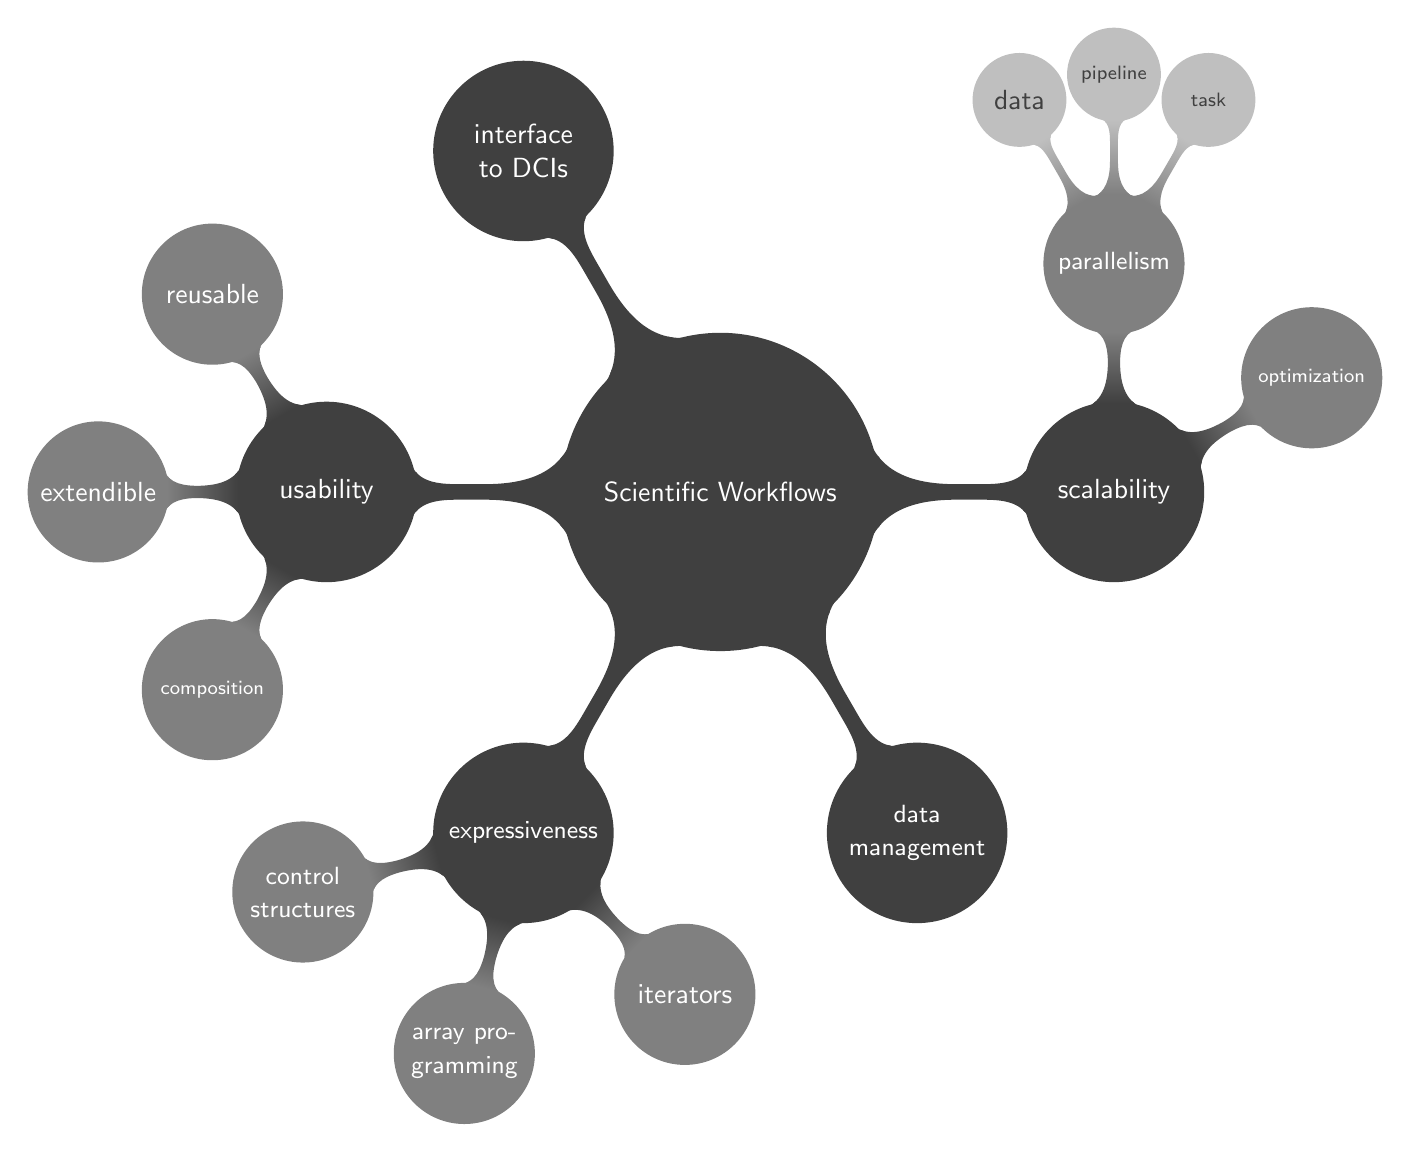
\begin{tikzpicture}[]
 \path[mindmap,concept color=darkgray,text=white,font=\sf]
 node[concept] {Scientific Workflows}
 [clockwise from=0]
 child[concept color=darkgray,font=\sf] {
 node[concept] {scalability}
 [clockwise from=90]
 child [concept color=gray,font=\sf] {
 node[concept] {\small{parallelism}}
 [clockwise from=120]
 child[concept color=lightgray,text=darkgray,font=\sf] {node[concept]{data}}
 child[concept color=lightgray,text=darkgray,font=\sf] {node[concept]{\scriptsize{pipeline}}}
	 child[concept color=lightgray,text=darkgray,font=\sf] {node[concept]{\scriptsize{task}}}
% 	 child[concept color=lightgray,text=darkgray,font=\sf] {node[concept]{\small{activity}}}
 }
 child[concept color=gray,font=\sf] { node[concept] {\scriptsize{optimization}} }
 }
 child[concept color=darkgray,font=\sf] { node[concept] {\small{data management}}}
 child[concept color=darkgray,font=\sf] {
 node[concept] {\small{expressiveness}}
 [clockwise from=-45]
 child[concept color=gray,font=\sf] { node[concept] {iterators} }
 child[concept color=gray,font=\sf] { node[concept] {\small{array programming}} }
 child[concept color=gray,font=\sf] { node[concept] {\small{control structures}} }
 }
 child[concept color=darkgray,font=\sf] {
 node[concept] {usability}
 [clockwise from=-120]
 child[concept color=gray,font=\sf] { node[concept] {\scriptsize{composition}} }
 child[concept color=gray,font=\sf] { node[concept] {extendible} }
 child[concept color=gray,font=\sf] { node[concept] {reusable} }
 }
 child[concept color=darkgray,font=\sf] { node[concept] {interface to DCIs} };
\end{tikzpicture}
\caption{A Taxonomy of the Features of Scientific Workflow Environments}
\label{fig:taxonomy}
\end{center}
\end{figure}

Figure \ref{fig:taxonomy} shows a taxonomy of SWE features studied in this
paper. We studied twenty SWEs from different scientific fields developed
worldwide. Some trends as observed in the approaches of the SWEs development
are noted below:

\begin{itemize}
 \item A recent surge in distributed computing approach of Cloud Computing has
     given rise to adoption of new enactment technologies. 

 \item SWEs tend to offer complementary properties which has led to several
     collaborations among the developing groups. Notable among these are the
     recent ones between Taverna and Galaxy \cite{mohamed-alaa-etal:2010} and
     Kepler and Pegasus \cite{mandal-deelman-etal:2007}.
 
 \item Collection oriented SWEs wherein arrays of data are treated as
     first-class entities has been seen a significant trend among the
     contemporary SWEs.
 
 \item A trend of increasing number of SWEs providing a script-based workflow
     composition interface solely or in combination with a visual interface in
     the form of GUI has been observed.
 
 \item Workflow systems originally developed for business domains have been
     introduced to scientific domains, such as BPEL and Trident.
\end{itemize}

In the present work we explore different dimensions of SWE paradigm. We study a
number of SWE implementations. While we see a number of implementations
dominant in areas suitable to their targeted applications, there is no single
SWE that could sufficiently fulfill the objectives of this work. There is a
lack of an SWE addressing the workflow expressibility and parallelism
requirements while at the same time targeting enactment within the Grid
Environment. Key features such as effective application data combinations or
array-based execution coupled with Grid centric execution are either missing or
partially available in the studied workflows. 

However, so far, from our study, we find Taverna as being the closest SWE that
can be a suitable candidate for our enactments. With this motivation, we get
into studying the details of the workings of the Taverna Workflow Environment. 

While many contemporary SWEs are studied in this survey, we are aware that this
is not an exhaustive list. Some other SWEs have been missed or omitted, notable
among them being: ICENI~\cite{furmento-mayer-etal:2002},
Calcium~\cite{caromel-henrio-etal:2008} and YML~\cite{delannoy-emad-etal:2006}.


% Bibliography
\bibliographystyle{ACM-Reference-Format-Journals}
\bibliography{sanebib}
%\nocite{*}
\end{document}

